%!TEX root = ../dokumentation.tex

\chapter{Automatische Beweisverfahren}
Automatische Beweisverfahren im allgemeinen dienen der automatisierten Überprüfung von logischen Schlussfolgerungen. Diese Verfahren werden insbesondere in der Mathematik eingesetzt, um neue Beweise auf Korrektheit zu prüfen. Um einen Beweis zu prüfen, wird dieser Formal definiert und anschließend von einem Computer überprüft. Diese werden unter einem Forschungszweig der künstlichen Intelligenz, dem \ac{ATP}, aktiv weiterentwickelt. Das folgende Kapitel stellt einige Beweisverfahren vor und zeigt Anwendungsgebiete dieser auf.

\section{Resolutionsverfahren}
Mit dem Resolutionsverfahren wird ähnlich dem Tableauxverfahren, aus der Verneinung einer logischen Formel ein Widerspruch abgeleitet. Es wird aus der Ausgangsformelmenge und der Annahmemenge eine sogenannte Resolvente abgeleitet, diese ist ebenfalls eine logische Formel. Die Resolvente hat die Eigenschaft einer notwendigen Bedingung für die Ausgangsformel. Das heißt die Ausgangsformel kann nur dann erfüllbar sein, wenn die Resolvente erfüllbar ist. Kann man also auf eine nicht erfüllbare (z.B. eine leere Formel) ableiten, hat man einen Widerspruch in der Ausgangsformel bewiesen. \cite{RN16}

Zur Ableitung einer Resolvente gibt es einige Regeln, welche hier nicht alle aufgeführt werden. Sei z.B. $\neg$A$\vee$K in der Ausgangsformelmenge und A die Annahme, so kann K als Resolvente abgeleitet werden. Im nächsten Schritt würde K als Element der Ausgangsformelmenge betrachtet werden und hieraus weitere Resolventen abgeleitet. \cite{RN16}

Dieses Verfahren hat starke Ähnlichkeiten zum Tableauxverfahren, verzichtet aber z.B. auf die Verzweigung der Beweissuche. Dies senkt die Laufzeitkomplexität und ist somit praktikabler für ein automatisches Beweisverfahren. Im Gegensatz zum Tableaux, kann einem Beweis allerdings weniger Intuitiv durch eine graphische Darstellung gefolgt werden.

Das grundlegende Verfahren ist momentan das Leistungsfähigste bekannte. Dies beweist der Theorembeweiser ``Vampire'', welcher der Gewinner der CADE ATP System Competition im Jahr 2019 (und den meisten Jahren zuvor) war. Dies ist ein jährlich abgehaltener Wettbewerb, bei dem Theorembeweiser auf ihre Leistungsfähigkeit im Bezug auf erfolgreich gelöste Probleme und Laufzeit verglichen werden. \cite{casc_atp_comp} Vampire basiert dabei auf einer Weiterentwicklung des Resolutionsverfahrens.

\section{Konnektionsmethode}
Die von Wolfgang Bibel vorgestellte Konnektionsmethode ist ein weiteres ATP-Verfahren. \cite{atp_bibel} Grundlage dieses Verfahrens ist die Darstellung der Formeln in Matrixform. Da Formeln für einen Beweis meist in der in \autoref{sec:grundlagen} vorgestellten Schreibweise vorliegen (z.B. $\alpha\vee\neg\beta$), ist der erste Schritt in diesem Verfahren die Umwandlung der Formel in Matrix Form.

Auf die genaue Definition der Umwandlungsregeln, wird im Rahmen dieser Arbeit verzichtet und stattdessen der Grundgedanke beschrieben. Eine etwas vereinfache Möglichkeit der Umwandlung, ist es die Formel zuerst in \ac{DNF} umzuwandeln. Eine Formel ist \ac{DNF}, gdw. die oberste Ebene der Formel ausschließlich aus konjunktiven Verknüpfungen, die untere Ebene aus disjunktiven Verknüpfen und (negierten) atomaren Aussagen. Die Formel $\alpha\vee(\beta\wedge\gamma)\vee(\alpha\wedge\neg\beta)$ ist ein Beispiel einer \ac{DNF} Formel. Liegt eine \ac{DNF} Formel vor, bilden die Elemente der konjunktiv verknüpften Formeln jeweils eine Spalte der Matrix. In \autoref{fig:example_matrix_formula}, ist die Formel $\alpha\vee(\beta\wedge\gamma)\vee(\alpha\wedge\neg\beta)$ in Matrix Form dargestellt. (Tatsächlich können in einem etwas komplexeren Verfahren Formeln in beliebiger Form in Matrixschreibweise umgewandelt werden)

\begin{figure}[H]
\begin{center}
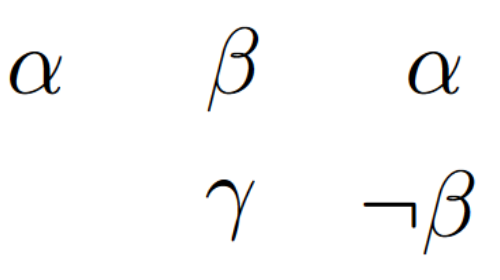
\includegraphics[scale=0.5]{images/example_matrix_formula.png}
\caption{Die Formel $\alpha\vee(\beta\wedge\gamma)\vee(\alpha\wedge\neg\beta)$ in Matrix Form.}
\label{fig:example_matrix_formula}
\end{center}
\end{figure}

Durch die Matrix können sogenannte Pfade gebildet werden. Vereinfacht, ist ein Pfad durch die Matrix eine Teilmenge der Elemente der Matrix, wobei aus jeder Spalte der Matrix genau ein Element auch Element des Pfades ist. (Auf die Behandlung von verschachtelten Matrizen wird der Einfachheit halber verzichtet.) Ein möglicher Pfad $\lbrace\alpha,\gamma,\neg\beta\rbrace$ durch die Beispielmatrix ist in \autoref{fig:example_matrix_path} dargestellt.

\begin{figure}[H]
\begin{center}
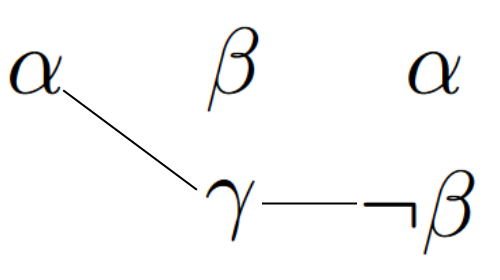
\includegraphics[scale=0.5]{images/example_matrix_path.png}
\caption{Pfad $\lbrace\alpha,\gamma,\neg\beta\rbrace$ durch die Matrix der Formel $\alpha\vee(\beta\wedge\gamma)\vee(\alpha\wedge\neg\beta)$.}
\label{fig:example_matrix_path}
\end{center}
\end{figure}

Eine Konnektion, ist nun eine Teilmenge eines Pfades der Form $\lbrace\alpha,\neg\alpha\rbrace$. Eine Menge von Konnektionen W wird als aufspannende Menge der Matrix F bezeichnet, gdw. für jeden Pfad p durch F ein w$\in$W existiert, sodass w$\subseteq$p. Eine Matrix wird als Komplementär bezeichnet, wenn für diese eine aufspannende Menge von Konnektionen existiert. Bibel bewies, dass jede komplementäre Matrix nur tautologische Formeln repräsentiert. \cite{atp_bibel}

Die Idee der Konnektionsmethode ist es also, für eine Matrix eine aufspannende Menge von Konnektionen bzw. deren Nichtexistenz aufzuzeigen. Der Algorithmus in der einfachsten Form läuft dann in folgenden Schritten ab:

\begin{description}

\item \textbf{1.} Erstelle Menge B aller Pfade durch F.

\item \textbf{2.} Wähle beliebige Konnektion k.

\item \textbf{3.} Betrachte Teilmenge von B, die nicht den Teilpfad k enthält. Ist diese leer, wurde mit den gewählten Konnektionen eine aufspannende Menge gefunden. Ist diese nicht leer, fahre mit 2 fort.

\end{description}

Der Vorteil dieser Methode ist, insbesondere im Vergleich mit einem auf Tableaux basierenden Beweis, die hohe Effizienz des Verfahrens.

\section{Anwendung von automatischen Beweisverfahren}
Neben den hier vorgestellten Verfahren, gibt es noch viele weitere \ac{ATP}-Verfahren. Die Verfahren finden Anwendung in vielen Open Source und kommerziellen Projekten zur Überprüfung der Korrektheit von mathematischen Schlussfolgerungen. Dies ist insbesondere wichtig in der Entwicklung von Mikroprozessoren. Firmen wie AMD und Intel verwenden automatische Beweisverfahren zur Verifizierung der Korrektheit von Division und anderen Operationen, die ein Mikroprozessor ausführen kann.

Eine andere Anwendung ist die Überprüfung von mathematischen Beweisen. In der Praxis werden diese allerdings eher selten Formal definiert und von einem automatischen Beweiser überprüft, da dies mit einem enormen Aufwand verbunden ist. Heutige mathematische Publikationen strecken sich oft über hunderte Seiten und eine für einen automatischen Beweiser verständliche Version ist meist deutlich länger, da hier viele Details hinzugefügt werden müssen, die in Publikationen oft als bekannt angenommen werden. Es gibt allerdings Anstrengungen, die (subjektiv) 100 wichtigsten mathematischen Theoreme zu formalisieren und von einem Computer überprüfen zu lassen. \cite{formalize_100_theorems} Zu den Theoremen gehören unter anderem der Satz des Pythagoras und Gödels Unvollständigkeitssatz. Die Überprüfung der Theoreme wird meist mit dem Programm \textit{HOL Light} durchgeführt. Wie der Name HOL (Higher Order Logic) bereits sagt, basiert dieser allerdings auf klassischer Logik höherer Ordnung, weshalb er nicht direkt mit den oben vorgestellten Verfahren verglichen werden kann.
